\chapter {Giới thiệu}
	
\section{Giới thiệu đề tài}
Khách hàng là nguồn sống của bất cứ cửa hàng, doanh nghiệp nào. Chính vì thế, chăm sóc khách hàng (CSKH) trở thành một trong những yếu tố sống còn và đòi hỏi rất nhiều đầu tư về công sức và tiền bạc. Có nhiều hình thức khác nhau để chăm sóc khách hàng như qua email, qua điện thoại, qua các diễn đàn trực tuyến, và qua tin nhắn trực tuyến.

Ở nước ta, việc giải đáp thắc mắc của khách hàng qua tin nhắn trực tuyến đang được ưa chuộng. Tuy nhiên, việc này còn thực hiện một cách thủ công và gặp nhiều khó khăn như: tốn rất nhiều thời gian và chi phí chi trả cho nhân viên chỉ để trả lời những câu hỏi đơn giản và giống nhau. Chính vì vậy, nhu cầu cấp thiết là cần một hệ thống điều khiển thông minh, tự động để mang lại hiệu quả cao hơn và Chatbot là một sự lựa chọn hoàn hảo. Cụ thể, tác dụng của Chatbot trong lĩnh vực chăm sóc khách hàng như sau:

\begin{itemize}
    \item Đưa thông tin chính xác tới từng tệp khách hàng.
    \item Trả lời tự động mọi câu hỏi của khách hàng đưa ra mọi lúc mọi nơi.
    \item Tăng sự tương tác của khách hàng và doanh nghiệp.
    \item Tự động chăm sóc khách hàng thường xuyên 24/7.
    \item Giảm chi phí đầu tư.
\end{itemize}

Chatbot chăm sóc khách hàng phù hợp với nhiều loại mô hình doanh nghiệp từ kinh doanh online (cung cấp thông tin sản phẩm, đưa ra các thông tin gợi ý, v.v.), hay là các nhà hàng, rạp chiếu phim (cung cấp các tùy chọn menu, chọn vị trí chổ ngồi, thanh toán, v.v.), và cũng được sử dụng nhiều trong lĩnh vực y tế, chăm sóc sức khoẻ.

Hiện nay, có rất nhiều hướng tiếp cận để xây dựng một Chatbot, tùy vào mục đích sử dụng. Trong đó, một phương pháp Chatbot khá phổ biến dựa trên quy tắc (rule-based), nó được huấn luyện bằng một hệ thống phân cấp các quy tắc được xác định trước, chuyển đổi các hành động của người dùng là đầu vào thành các hành động đầu ra của Chatbot. Vì vậy, với hệ thống này nó không thể phản hồi với các mẫu đầu vào hay các từ khóa không phù hợp với các quy tắc hiện có. Và với mỗi mẫu đầu vào, nó sẽ có một quy tắc phản hồi cố định, các quy tắc này giúp cho hệ thống làm việc được chặt chẽ. Tuy nhiên, các hành vi sẽ bị lặp đi lặp lại, dẫn tới một hệ thống cứng nhắc và nhàm chán. Một phương pháp khác, hiện thực một hệ thống hội thoại tự do hơn như \textit{Sequence To Sequence}. Nó huấn luyện để cho tác nhân tự tạo ra các câu trả lời và có khả năng xử lý được các câu mà nó chưa từng gặp. Tuy nhiên, nó không theo dõi được và hướng hội thoại theo cùng một ngữ cảnh. Trong luận án này, đề tài hướng đến một phương pháp mới, hiện đại, và phát triển ngày càng mạnh mẽ hiện nay, là phương pháp học tăng cường (reinforcement learning). Phương pháp này nó mô hình hóa cho tác nhân nên thực hiện các hành động sao cho tối ưu hóa phần thưởng tích lũy. Vì thế, sau quá trình huấn luyện, các tác nhân nó vẫn theo được các quy tắc ban đầu đặt ra, hướng hội thoại vào cùng một ngữ cảnh. Và tùy vào trạng thái hiện tại của hội thoại, tác nhân phản hồi linh hoạt hơn, có khả năng vượt ra ngoài quy tắc ban đầu được xây dựng.

\section{Mục tiêu và các giai đoạn thực hiện của đề tài}
\label{sec:muctieu}
Trong phạm vi nghiên cứu của đề tài này, tập trung xây dựng một hệ thống hội thoại tự động có thể tư vấn cho khách hàng thông tin về các sản phẩm thời trang như quần áo, váy đầm, v.v. Cụ thể, hệ thống bao gồm các tính năng sau:

\begin{itemize}
    \item Cung cấp nguồn dữ liệu tin cậy để Chatbot có thể tư vấn đầy đủ và chính xác cho người dùng.
    \item Hiểu được ý định, nhu cầu của người dùng khi họ tham gia hội thoại với Chatbot, trích xuất được các thông tin mà người dùng cung cấp để truy vấn chính xác, thoả mãn yêu cầu của người dùng.
    \item Thỏa mãn, hoàn thành được yêu cầu của người dùng khi tham gia cuộc hội thoại. Mang lại sự hài lòng tốt nhất có thể cho người dùng.
    \item Giao tiếp với người dùng một cách linh hoạt, bám sát với luồng hội thoại để mang lại trải nghiệm tốt nhất có thể cho người dùng.
\end{itemize}

Để có thể đạt được những tính năng trên, cần xác định một số công việc phải giải quyết như sau:

\begin{itemize}
    \item Tìm kiếm và thu thập dữ liệu phù hợp với nội dung đề tài. Lọc nhiễu, trích xuất các thông tin cần thiết để lưu trữ vào cơ sở dữ liệu phục vụ cho nhu cầu truy vấn cho Chatbot.
    \item Khảo sát nhu cầu của người dùng khi cần được tư vấn thông tin sản phẩm, từ đó xây dựng được các kịch bản tư vấn cho người dùng.
    \item Huấn luyện cho hệ thống, sử dụng mô hình học tăng cường, để có thể đưa ra quyết định cho mỗi hành động khi giao tiếp với người dùng một cách tốt nhất.
    \item Xây dựng các hệ thống đi kèm khác để hỗ trợ cho việc giao tiếp với người dùng như truy vấn dữ liệu chính xác, trả về đúng thông tin người dùng mong muốn.
    \item Xây dựng bộ sinh câu phản hồi của Chatbot với ngôn từ tự nhiên tạo cảm giác thoải mái cho người dùng.
    \item Xây dựng với bộ giao diện ứng dụng thân thiện, dễ sử dụng.
\end{itemize}

\section{Các giai đoạn thực hiện}
Với những mục tiêu đã đề ra ở mục \ref{sec:muctieu}, đề tài được thực hiện qua các giai đoạn như sau:

\begin{itemize}
    \item \textbf{Giai đoạn 1:} Tìm kiếm và thu thập các thông tin về sản phẩm thời trang để thiết kế ra các hoạt động mà Chatbot có thể hỗ trợ.
    \item \textbf{Giai đoạn 2:} Khảo sát và thu thập các thông tin từ người dùng để thiết kế ra các ý định của người dùng.
    \item \textbf{Giai đoạn 3:} Thiết kế hệ thống và định nghĩa cách kiểm thử, đánh giá hệ thống.
    \item \textbf{Giai đoạn 4:} Xây dựng mô hình huấn luyện gồm các bộ sinh phản hồi, bộ quản lý hội thoại, bộ mô phỏng người dùng và lỗi.
    \item \textbf{Giai đoạn 6:} Xây dựng các thành phần cấu thành ứng dụng Chatbot đơn giản. Đồng thời, tổng hợp các thành phần còn lại thành một hệ thống hoàn chỉnh.
    \item \textbf{Giai đoạn 7:} Tiến hành kiểm thử và đánh giá hệ thống.
\end{itemize}

% Thời gian cụ thể thực hiện được mô tả như sau:

% \begin{center}
%     \begin{figure}[h!]
%         \begin{center}
%          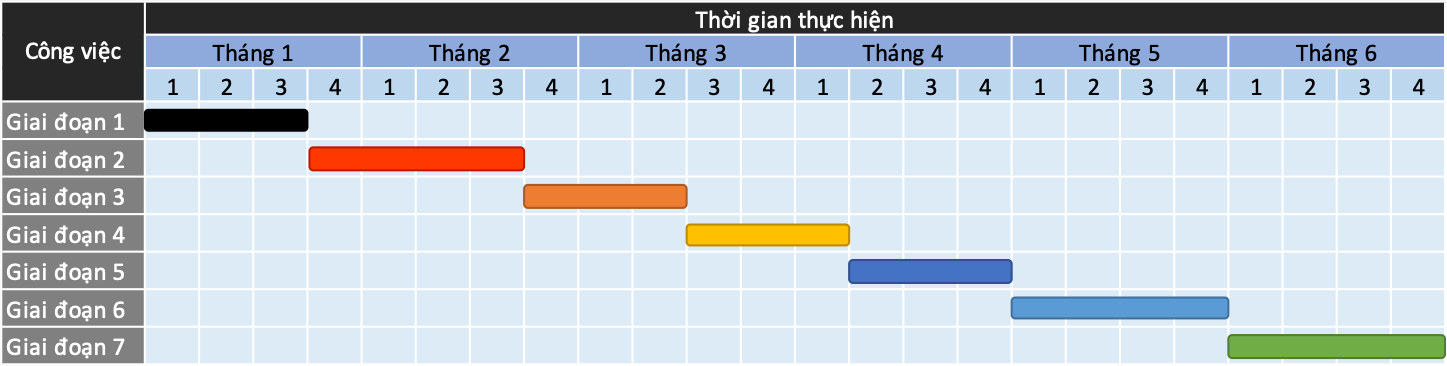
\includegraphics[scale=0.63]{chapter4.5/img/timeline.png}
%         \end{center}
%         \caption{Thời gian thực hiện đề tài}
%     \end{figure}
% \end{center}

\section{Giới hạn của đề tài}
\label{sec:scope}
Các nhu cầu của khách hàng trong lĩnh vực tư vấn thời trang là rất phong phú nên việc đáp ứng hết tất cả nhu cầu là rất khó khăn. Vì vậy, trong đề tài này tôi sẽ cố gắng đáp ứng được những nhu cầu đã được định nghĩa.

Trong đề tài này, chỉ tập trung vào việc nghiên cứu và sử dụng mô hình học tăng cường huấn luyện cho Chatbot để mang lại độ chính xác lẫn tự nhiên có thể chấp nhận được, mang lại trải nghiệm thoải mái cho người dùng.

Đồng thời, xây dựng bộ mô phỏng người dùng và tạo lỗi để tự động sinh ra các mẫu hội thoại có tính tự nhiên và dùng nó để huấn luyện cho Chatbot.

Ngoài ra, đề tài còn xây dựng ứng dụng Chatbot với giao diện đơn giản có thể giao tiếp với người dùng dễ dàng.

\section{Cấu trúc luận văn}

\begin{itemize}
    \item \textbf{Chương 1:} Giới thiệu tổng quan về đề tài, mục tiêu, giới hạn và các giai đoạn thực hiện đề tài.
    \item \textbf{Chương 2:} Trình bày một số công trình có liên quan tới đề tài.
    \item \textbf{Chương 3:} Trình bày các kiến thức nền tảng có liên quan tới đề tài. Và cách hoạt động của nó trên bài toán của đề tài.
    \item \textbf{Chương 4:} Trình bày phương pháp giải quyết bài toán: mô tả về kiến trúc hệ thống, quá trình huấn luyện mô hình học tăng cường.
    \item \textbf{Chương 5:} Trình bày các công cụ và công nghệ sử dụng để giải quyết bài toán.
    \item \textbf{Chương 6:} Trình bày cách thức hiện thực hệ thống.
    \item \textbf{Chương 7:} Trình bày cách thức kiểm thử và đánh giá hệ thống.
    \item \textbf{Chương 8:} Tổng kết quá trình thực hiện luận văn, những hạn chế và hướng phát triển.
\end{itemize}
